\section{Smart Homes}
Another trend that utilizes the concept of IoT is smart homes which are homes that are, 
to some degree, automated by utilization IoT devices. 
The devices used for smart homes differ greatly from wearables as they are usually stationary. 
The concept of smart homes have been around for a while and numerous homes have already integrated some of these smart devices. 
A good example of a high-end smart home is Bill Gate's mansion in Medina, Washington \cite{billgatehouse}.
This \$100 million house have sensors to adjust each room's temperature and lighting, 
and have speakers behind the wallpaper that follows you from room to room. 
The artwork in the house is mostly digital and can be changed by pressing a button. 
One can only imagine what other technology is being used in that house. 

However, that is a rather extreme example of a smart home. 
Ordinarily, the devices found in smart homes are common items that has been connected to the Internet for wireless control.
Common devices that are found in smart homes include, but are not limited to, 
coffee machines, washers and dryers, thermostats, sound systems and locks. 
However, only few devices have really gained ground for the common user and few homes are automated.
One of the most commonly found IoT in homes are the Nest thermostat \cite{NEST}. 
This thermostat senses when you are around and when you are not to control the climate inside to save energy and thus money.
Unlike a lot of smart devices that are made to make your life a little easier, such as an automated coffee machine, 
the Nest thermostat helps you save money which is likely the reason for it popularity. 
Furthermore, the newest version (as of October 2015) allows you to connect other IoT devices to the thermostat. 
The Nest thermostat is thus starting to solve what is probable the greatest problem with smart homes (and IoT in general), 
and why they have not become popular yet: Lack of interconnectivity between IoT devices. 
This problem leads us to what is known as smart hubs. 

\subsection{Smart Hubs}
A smart hub is a device, or service, that implements several communication protocols used by IoT devices, 
and gives the user a single protocol or interface. 
The goal of a smart hub is to make the connected devices able to communicate. 

\begin{figure}[!htb]
    \centering
    \tikzstyle{block} = [draw, rectangle, minimum width=3cm, minimum height=1cm]
\tikzstyle{myarrows}=[line width=0.5mm,triangle 60-triangle 60]
\begin{tikzpicture}
\node [block] (internet) at (0,0) {Internet};
\node [block] (zigbee) at (-5, 0) {Zigbee Network};
\node [block] (zwave) at (-2.5, 2.5) {Z-Wave Network};
\node [block] (services) at (2.5, 2.5) {Application Services};
\node [block] (wifi) at (5, 0) {WiFi};
\node [block] (bluetooth) at (0, -2.5) {Bluetooth};

\draw [myarrows] (internet) -- (zigbee);
\draw [myarrows] (internet) -- (zwave);
\draw [myarrows] (internet) -- (services);
\draw [myarrows] (internet) -- (wifi);
\draw [myarrows] (internet) -- (bluetooth);
\end{tikzpicture}
    \caption{Architecture of IoT network}
    \label{fig:IoTProtocols}
\end{figure}

\subsubsection{Common Protocols for IoT}
\todo[author=Thalley]{Insert figure illustrating this}
There is a range of different protocols that are being used for various smart devices. 
We will not get into much detail with these protocols, 
but we demonstrate how many different there are and why communication is a problem.
\begin{table}
   \begin{description}
       \item[Protocol:] ZigBee
       \item[Used by:] Samsung, Jasco, Smartenit, FortrezZ and others
       \item[In products:] SmartThings Hub, thermostats, door sensors, light bulbs, etc.\\
       
       \item[Protocol:] Z-Wave
       \item[Used by:] FortrezZ, GE, Intermatic, Leviton, Aeon Labs, Evolve and others
       \item[In products:] Thermostats, wall outlets, door locks, door and window sensors, etc.  \\
       
       \item[Protocol:] WiFi (IEEE 802.11)
       \item[Used by:] Nest, Philips, Samsung, Bose, D-link and others
       \item[In products:] Thermostats, speakers, light bulbs, motion sensors, fitness trackers, camera, etc. 
    \end{description}
    \caption{Protocols used by various IoT devices}\label{table:iotprotocols}
\end{table}

Aside from the protocols in \Cref{table:iotprotocols}, 
there are several others messaging protocols such as MQTT, CoAP and XMPP used by various devices. 

A smart hub should thus not only be able to communicate with the devices, 
but also be able to transform the data to a single format and give easy access to it. 

\subsubsection{Smart Hubs on the Market}
The requirements for smart hubs have gained the attention of several large companies and even more smaller companies, 
all competing to be center of future smart homes. 
One of the mature commercial available smart hubs is the Samsung SmartThings Hub\cite{SMARTTHINGS}. 
The SmartThings Hub is a standalone device that supports the Z-Wave, ZigBee and WiFi protocols, 
and provides a smartphone application or a Representational State Transfer (REST) interface. 
The SmartThings Hub has been tested and is compatible with more than 150 devices as of October 2015,
but with support for the aforementioned protocols and a REST interface, this number is in practice higher.  
The price for such a hub is \$99, which is, compared to the prices for some of the compatible devices, very affordable. 
A more detailed description of the Samsung SmartThings Hub can be found in \Cref{sec:smartthings}. 

Samsung is, however, not the only company selling smart hubs. 
Microsoft has been working on their HomeOS\cite{HOMEOS}, Apple has their HomeKit\cite{HOMEKIT} and Google recently announced Brillo\cite{BRILLO}. 
While these products differ in terms of architecture, descriptions (operating system contra hub) and availability,
they all share the same goal of giving a centralized control of smart devices. 

There are also other open source alternatives such as openHAB\cite{OPENHAB}, 
where you simply setup your own server running the open sourced code and control the devices through that. 
The advantage here is of course the price (free) and the possibility of adding new unsupported products. 

\Cref{table:smarthubs} gives a short overview of some of the available or coming smart hubs. 
\begin{table}
    \centering
    \begin{tabular}{l l}
        Company                           & Product Type \\ \hline
        openHAB\cite{OPENHAB}             & Employ open source code on own server \\
        Open Source Automation\cite{OSA}  & Employ open source code on own server \\
        OpenRemote\cite{OPENREMOTE}       & Employ open source code on own server \\
        Apple\cite{HOMEKIT}               & HomeKit Framework \\
        Samsung\cite{SMARTTHINGS}         & SmartThings Hub: A standalone device that costs \$99 \\
        Microsoft\cite{HOMEOS}            & HomeOS: An operating system that runs on a server \\
        Google\cite{BRILLO}               & Project Brillo: An operating system that runs on a server
    \end{tabular}
    \caption{An overview of home automation hubs from different companies}
    \label{table:smarthubs}
\end{table}

\subsection{Control of Smart Homes}
While smart hubs let different smart devices communicate, 
they are not meant to be a control panel for smart homes (although some, such as HomeOS, is designed as such).
To control the devices connected to a smart home, or standalone smart devices, 
most vendors offer some sort of smartphone application that gives the consumer a basic interface to control the device, set rules for it and so on.
This is for example the case with the Samsung SmartThings hubs. 

An alternative to such an application could be the Logitech Harmony Remote\cite{HARMONYREMOTE}, 
which is a universal remote that can connect to over \num{270000} devices (smart and dumb). 
It comes either as a standalone remote control or connected with a hub. 

Gesture control is a newer and more advanced way of controlling a smart home. 
A company known as Reemo\cite{Reemo}, formerly Playtabase, has created a way of controlling smart devices by gestures. 
They have developed a wearable devices, located on the wrist, that allows user to point at a device, 
and then perform a pre-programmed gesture that corresponds to a certain action for that device. 
A small received has to be placed near the devices that you want to control, 
and it is this received that you have to point to as depicted by \Cref{fig:reemo}. 
The pointing will, however, only work if the device is within line of sight. 

%Thalley: Skal vi bare skrive ``Reemo'' i stedet for en url som source?
\begin{figure}[!htb]
    \centering
    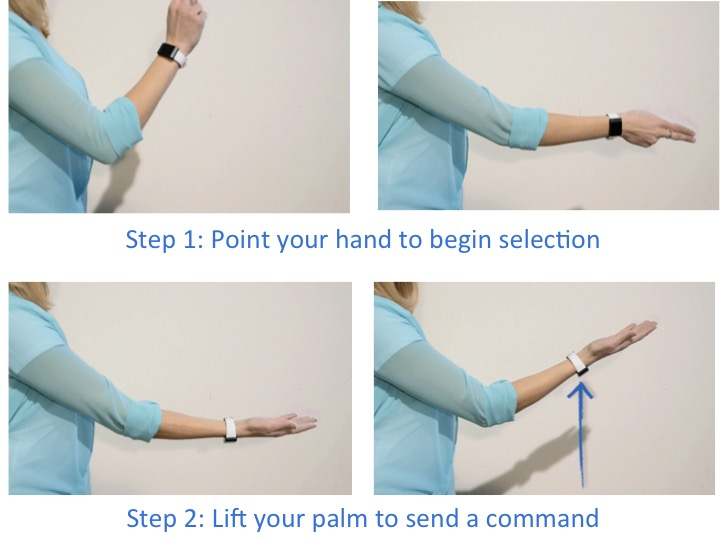
\includegraphics[width=0.8\textwidth]{images/Reemo}
    \caption{How Reemo gesture control works. Source: \url{http://www.getreemo.com/projects/}}
    \label{fig:reemo}
\end{figure}

Unfortunately they have not disclosed any details regarding the technology, 
how the receivers know which receiver you are pointing at or how the devices are controlled. 
The company and the product is also still in a development phase, 
so the product is not commercialized yet but have been in development since mid-2014.

These are the most common and/or most intuitive ways of controlling smart devices. 
The question is which is ``the best'', or rather, which method is the wanted way of controlling the devices.
\Cref{tbl:smartcontrol} summaries the aforementioned 3 ways. 

\begin{table}[!htb]
    \centering
    \parbox[t][][t]{0.3\textwidth}{
        \textbf{Smartphone Application}\\
        \textbf{Pros:} Easy control of smart devices if the smartphone is usually carried or always near. 
                       Applications are usually available from vendors. 
                       Easy to get updates to the software. \\
        \textbf{Cons:} Requires a smartphone nearby to control. 
                       An overhead of unlocking phone, opening application and selecting device and action.
    }\quad
    \parbox[t][][t]{0.3\textwidth}{
        \textbf{Remote Control}\\
        \textbf{Pros:} Easy control of smart devices if the remote is usually carried or always near. \\
        \textbf{Cons:} Requires a remote control nearby to control (usually not very expensive). 
                       An overhead of selecting device and action.
    }\quad
    \parbox[t][][t]{0.3\textwidth}{
        \textbf{Gesture Control}\\
        \textbf{Pros:} Wearables are usually worn and grants easy control of applications by gesture.
                       Intuitive way of controlling devices (gestures imitates regular actions).
                       Easy to get updates to the software. 
                       No overhead of opening an application\\
        \textbf{Cons:} Requires a wearable to control. 
                       Have to remember gestures.
                       Must be in line of sight. 
    }
    \caption{Ways of controlling smart devices}
    \label{tbl:smartcontrol}
\end{table}

Each way has its pros and cons. 
A survey of 37 people showed that \perc{76} found gestures to be a natural way of controlling devices, 
while \perc{8} found it unnatural and the remaining left the question unanswered\cite{Kela2006}. 
This survey shows that users would rather have gesture for control, 
rather than the bother of always using their smartphone or remote for control.  
A product such as Reemo is a good way of controlling smart devices. 
However, as mentioned, it has a downside that the objects have to be in line of sight. 
If this restriction could be removed, it would improve this method. 

%%% Local Variables:
%%% mode: latex
%%% TeX-master: "../../master"
%%% End:
